\documentclass[20 pts]{article}
%\usepackage{xeCJK}
\usepackage{amsfonts}
\usepackage{amssymb}
\usepackage{csvsimple}
\usepackage{caption}
\usepackage{longtable}
\usepackage{amsmath}
\usepackage{bm}
\usepackage{graphicx}
%\setCJKmainfont{SimSun}
\title{Deterministic Interleaver Design for Turbo Codes} 
\author{Kwame Ackah Bohulu, 1631133}
\date{22-06-2017}


\begin{document}
\maketitle
\newpage
\section{Abstract}
input weight 2m error events with the distance between the bit '1' seperated by a 
multiple of
the componet codes cycle length ($a-\tau$ seperated input weight 2m error events) 
tend to produce low-weight turbo codewords if present
in both component codes. In this research paper, we introduce a 
method for designing deterministic
interleavers for turbo codes in such a way that $a-\tau$ seperated input weight 2m 
error events in 
the first component encoder are not mapped unto the second component encoder. 
Using
this method, we find good interleavers for specified frame lengths and component 
codes. The performance of the designed interleavers is tested against the Quadratic 
Permutation Polynomial (QPP) Interleaver and is shown to be better especially for long
frame sizes.

\section{Introduction}
Turbo Codes are amongst the class of capacity approaching FEC codes that were 
discovered in 1993 by Claude Bearoux. They are constructed by the parallel 
concatenation of 2 Recursive Systematic Convolutional (RSC) Encoders via an 
interleavers. Diagram for 


Decoding of Turbo codes is done using the Turbo Decoder. It is made up 2 Soft 
Input Soft 
Output (SISO) Decoders.
The interleaver plays a very important role in Turbo codes as it reduces the number of
 low-weight codewords(multiplicity) of the Turbo code [4]. However, the existence of 
 the low-weight codewords causes the turbo codes to have a high error floor in the 
 high SNR region. A lot of research has been done concerning interleavers for 
 turbo codes and they are generally put into 2 groups, Random and 
 Deterministic interleavers.
\paragraph{}
Turbo codes implemented using Random interleavers have been shown to have good
 performance, especially for large frame sizes [3]. The disadvantage of using 
 Random interleavers stems from required use of interleaver tables in both the 
 encoder and decoder, which is undesirable in many applications. 
 Deterministic interleaver
  on the other hand require no such interleaver tables and the logic behind interleaving
   and deinterleaving can be executed by means of algorithms. Due to this advantage, 
   a lot of Turbo codes employ Deterministic interleavers in their construction. Most 
   noticable amongst these is the Quadratic Permutation Polynomial (PP2) 
   interleaver [3]
    which is used in LTE applications.
\paragraph{}
Despite this advantage, Deterministic interleavers that outperform Random interleavers,
 especially for large frame sizes have yet to be discovered. The aim of this research is
  to design an interleaver that has a performance that is at least as good as that of 
  random 
  interleavers for large frame sizes. 

\subsection{Turbo Encoding and Decoding}
The Turbo encoder is shown in figure (\ref{TC}).

\begin{center}
\begin{figure}[h!]
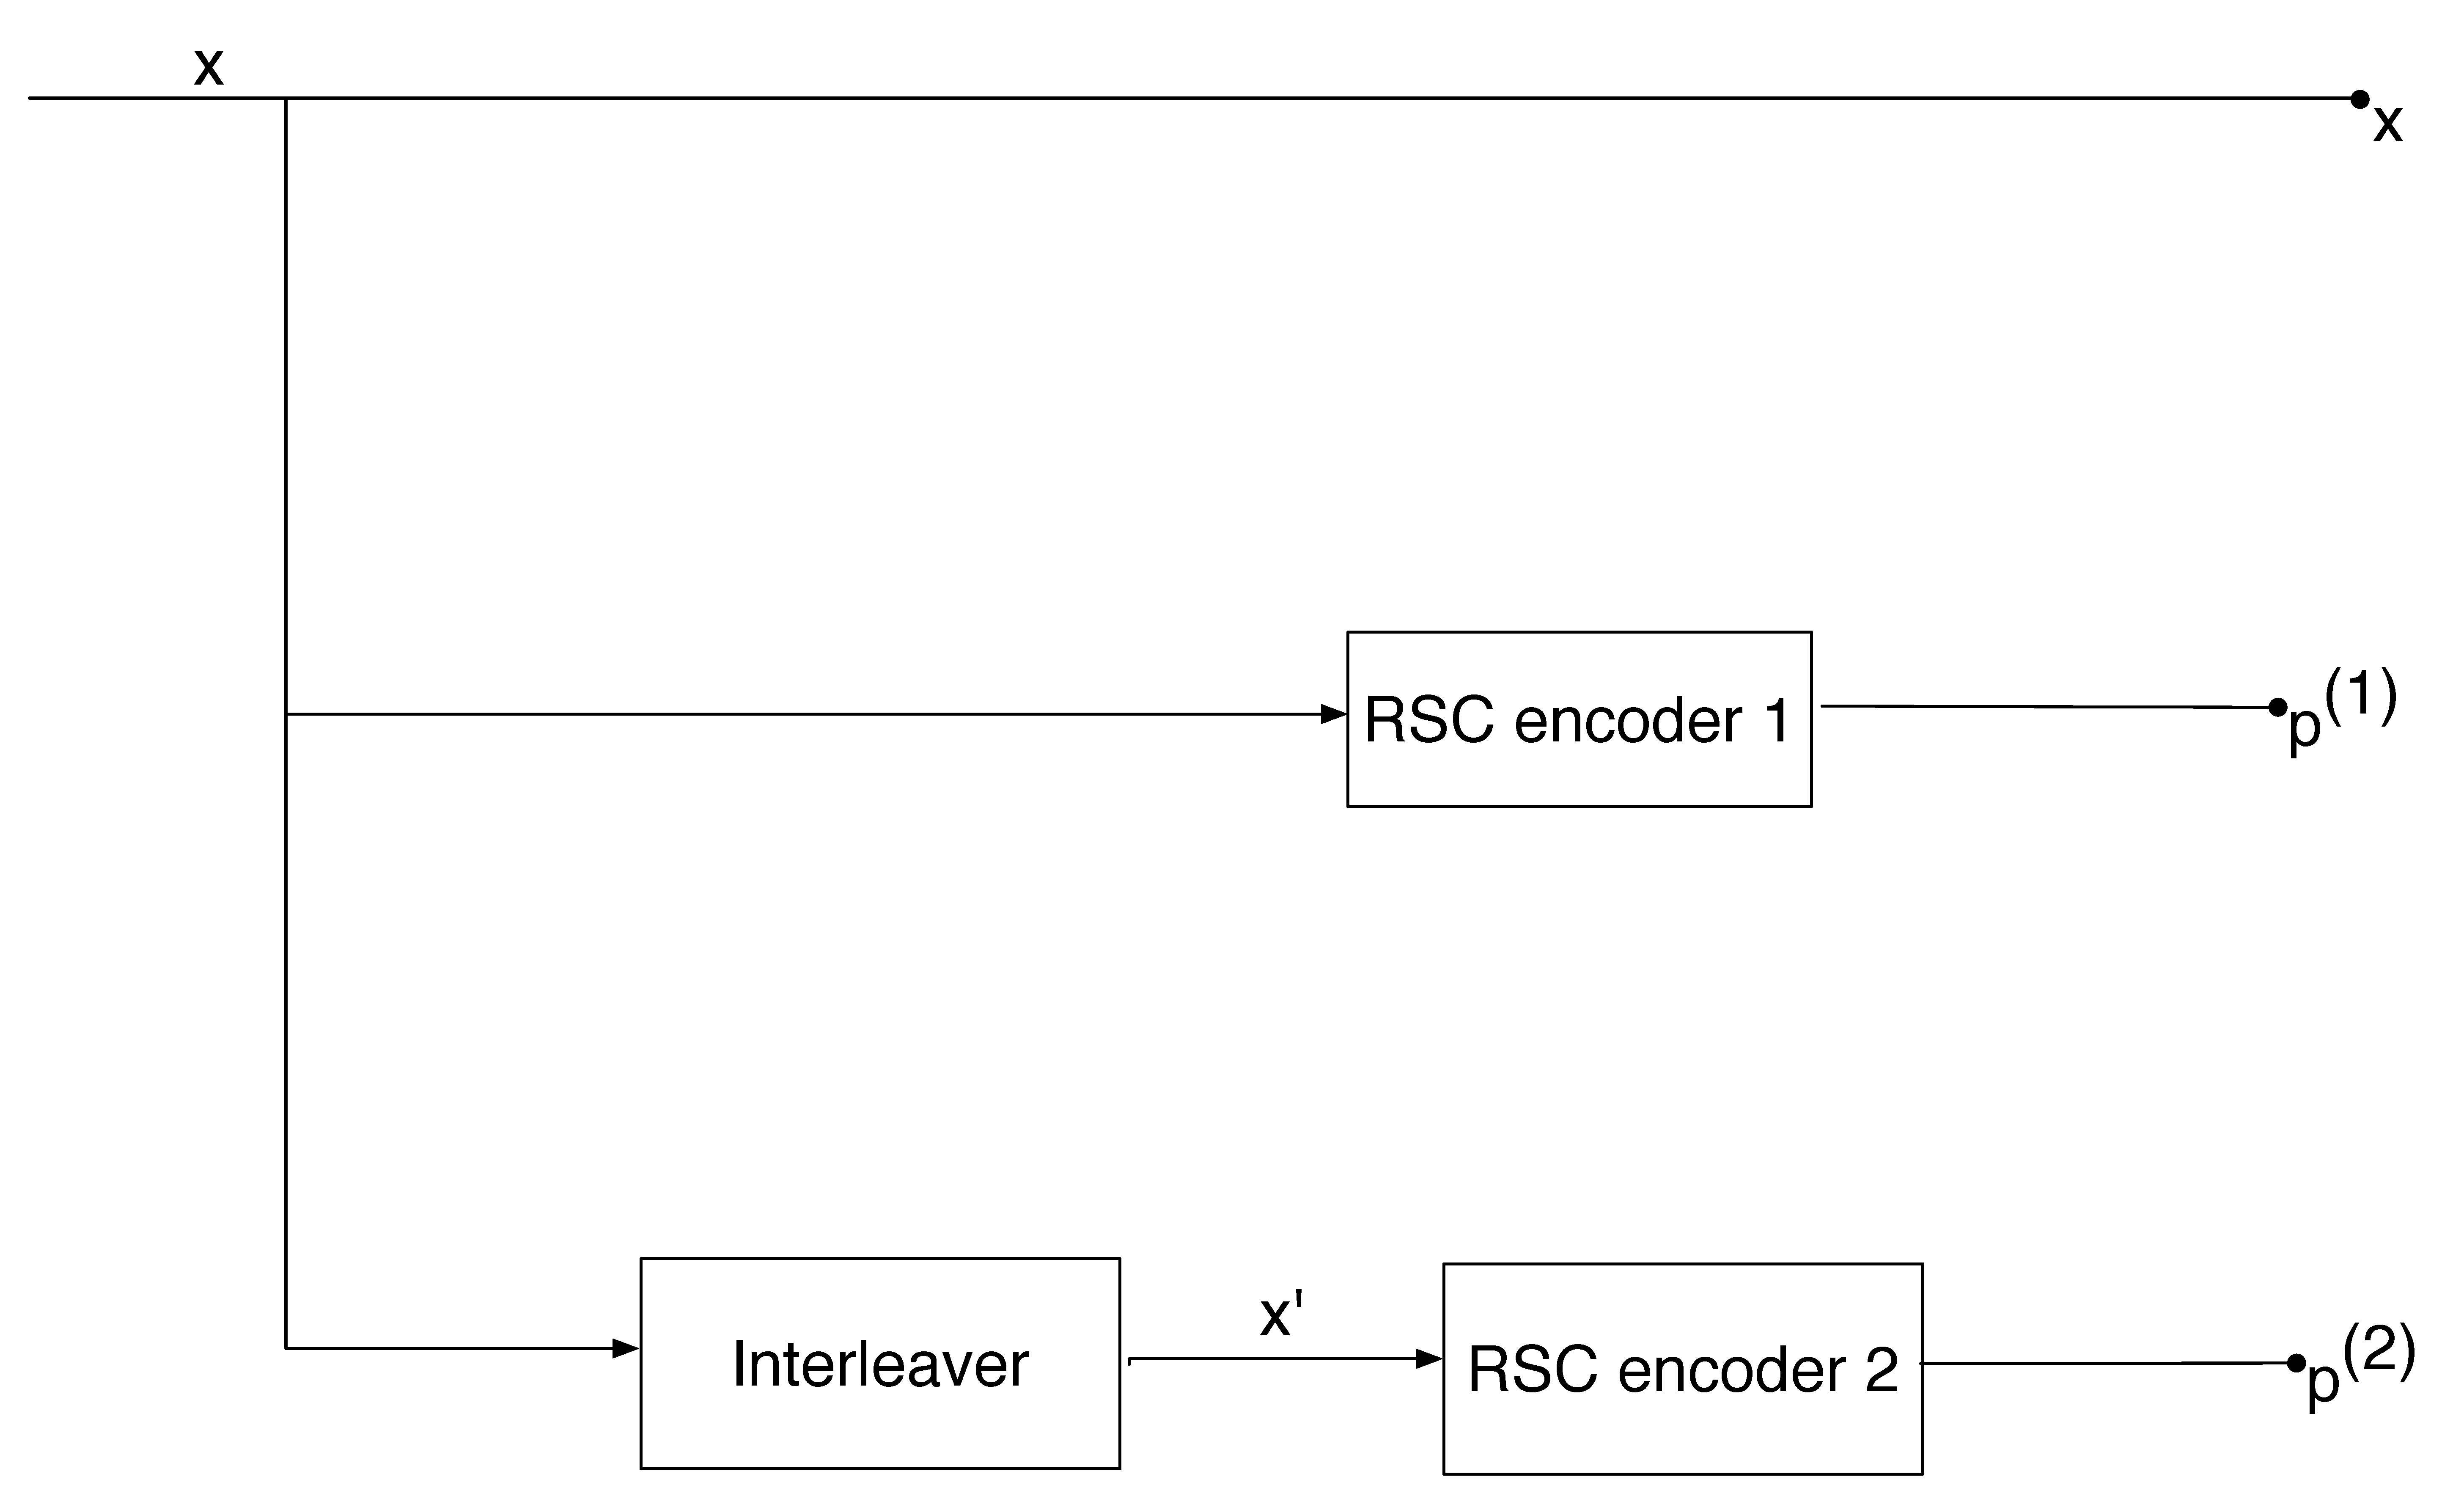
\includegraphics[width=8cm]{TurboEncoder.pdf}
\caption{Turbo Encoder}
\label{TC}
\end{figure}
\end{center}
\paragraph{}The component encoders (CEs) used are identical (N+$m_{RSC}$, N) 
RSC encoders with the 
generator matrix given in octal form $\frac{d}{e}$ where e is the feedback vector 
,d is
the feedforward vector and $m_{RSC}$ is the memory order of the RSC encoder. 
In our
encoding scheme, we wish to return the CEs to the all-zero state.This is acheived by
using $m_{RSC}$ non-zero tail bits. The turbo encoding process is as follows.
The binary input information (systematic) 
sequence $\mathbf{u}=\{u_1, u_2,...,u_{N-1}, u_N \}$ of
 length N is fed into each CE. The upper CE receives the
  input as is and produces the upper parity bit sequence 
  $\mathbf{v}=\{v_1, v_2,...,v_{N-1}, v_N,...,v_{N+m_{RSC}} \}$
  of length N+$m_{RSC}$ . The input to
  the lower CE is an interleaved version of the input information sequence 
  $\mathbf{u}'=\{u'_1, u'_2,...,u'_{N-1}, u'_N \}$. This is used to generate the 
  lower parity bit sequence 
  $\mathbf{v}'=\{v'_1, v'_2,...,v'_{N-1}, v'_N,...,v'_{N+m_{RSC}} \}$ also
  of length N+$m_{RSC}$. The output rate of the turbo code using this encoding
  scheme is $\frac{N}{3N+2m_{RSC}}$. The systematic, upper and lower parity bits 
  are multiplexed and modulated using BPSK and transmitted over the AWGN channel.

\paragraph{}
Decoding of turbo codes is done using the turbo decoding algorithm. This algorithm
is based on the iterative use of the BCJR algorithm or variations of it. 
In this research we
use the Max-Log-APP algorithm as described in [].

Assuming BPSK modulation and transmission over the AWGN channel
the a posteriori LLR values are calculated using the equation below.
\begin{equation}
L(u_i)=L_cy^s_i + L_a (u_i) + L_e(u_i)
\label{LLR}
\end{equation}
The meaning and definitions of all variables related to (\ref{LLR}) are summarized in
Table \ref{LLR}.

\begin{table}[h!]
\begin{center}
 \begin{tabular}{|| c | c | c | c ||} 
 
 \hline
 variable & definition & formula & initial values  \\ [0.5ex] 
 \hline\hline
 $L_cy^s_i$ & 0 0 $\rightarrow$ 1 0 & 1 0 $\rightarrow$ 1 1 & 1 1 $\rightarrow$ 0 1  \\ 
 \hline
 $L_a (u_i)$  & 0 0 $\rightarrow$ 0 0 & 0 0 $\rightarrow$ 1 0 & 1 0 $\rightarrow$ 0 1  \\ 
 \hline
  $L_e(u_i)$& 0 0 $\rightarrow$ 1 0 & 1 0 $\rightarrow$ 0 1 & 0 1 $\rightarrow$ 1 0  \\ [1ex] 
 \hline
 
\end{tabular}
\label{T1}
\end{center}
\label{T1}
\caption{$d_k = 0$}
\end{table}

The Turbo decoder is shown in Figure \ref{TD}.
\begin{figure}[h!]
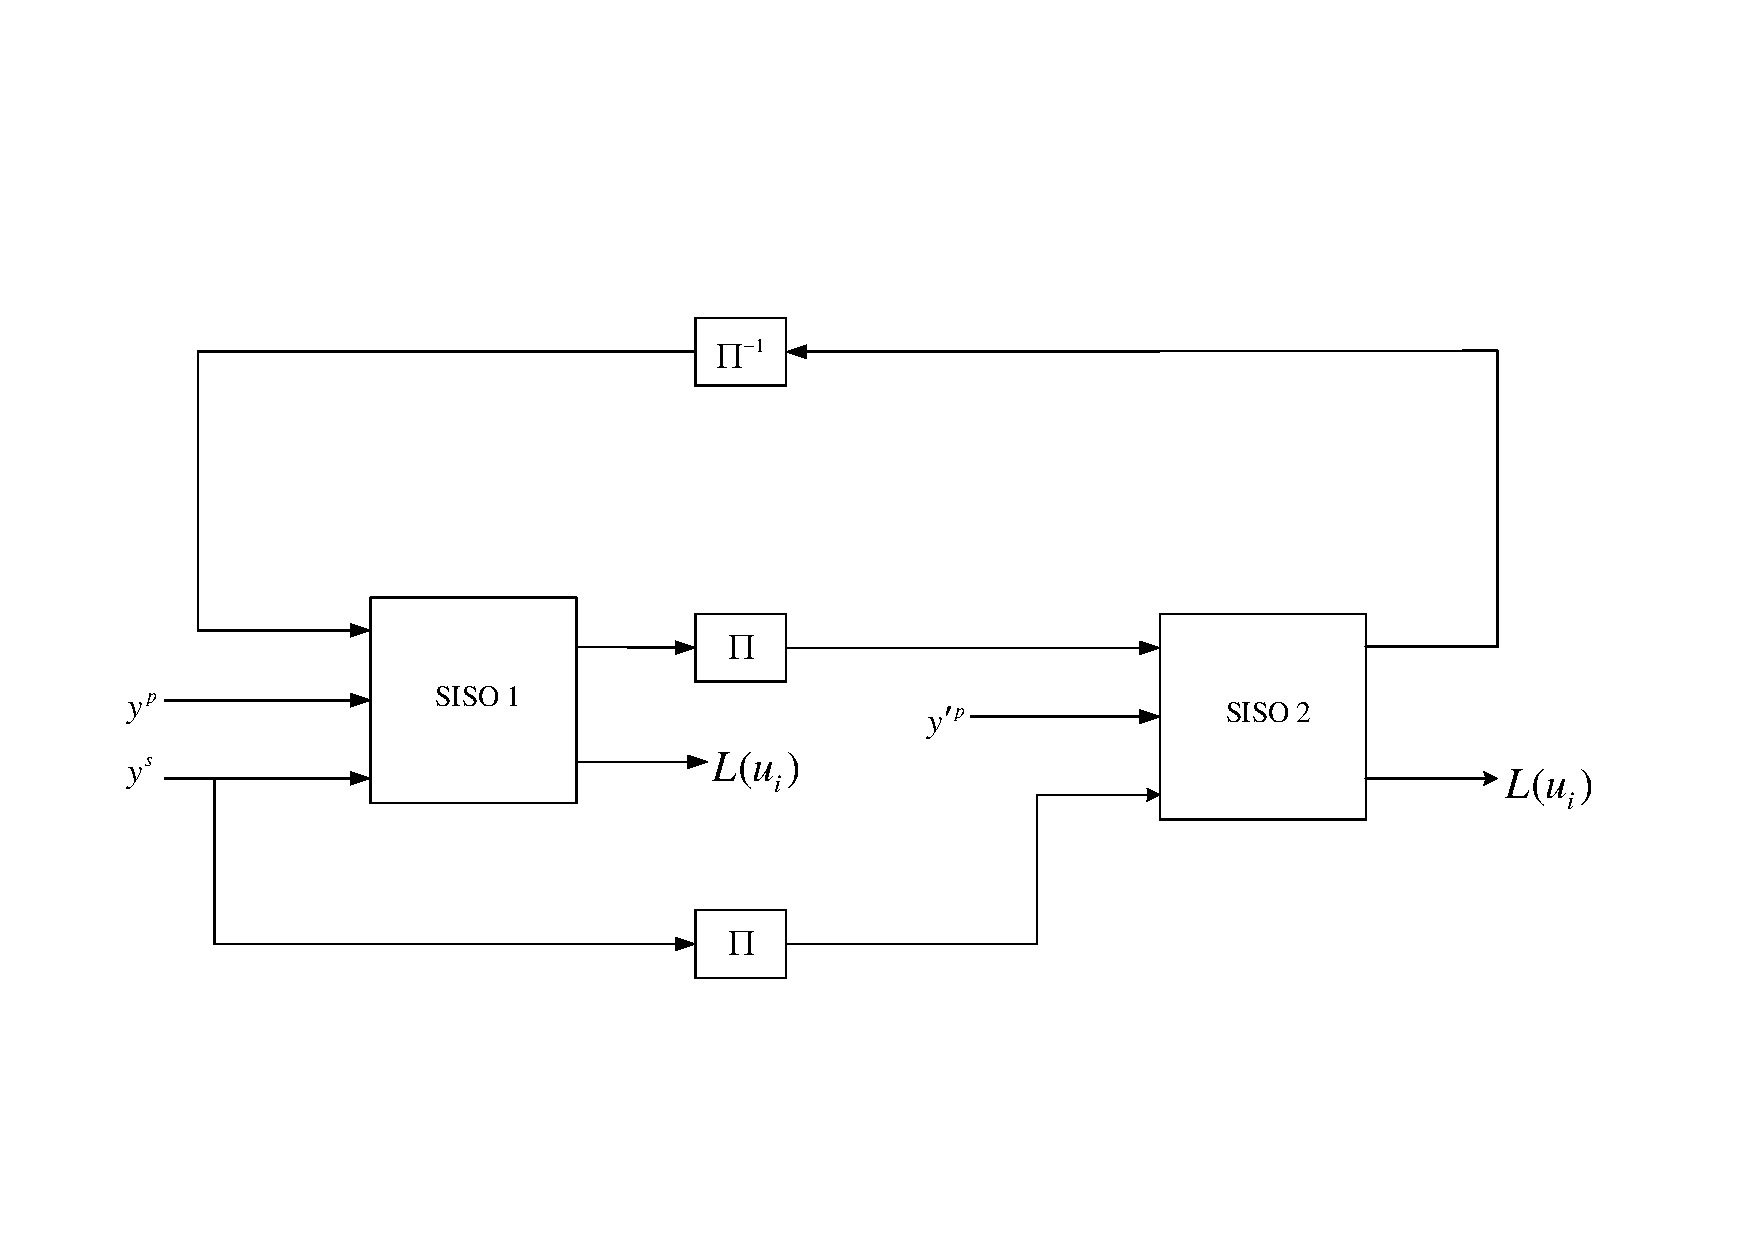
\includegraphics[width=10cm]{D1.pdf}
\caption{Turbo Decoder}
\label{TD}
\label{図2}
\end{figure}
it utilises 2 Soft Input Soft Output (SISO) decoders(one for each encoder) 
connected in such
a way that the $L_e(\mathbf{u})$ from one encoder is fed into the other as
 $L_a(\mathbf{u})$.
 \paragraph{}
 The turbo code transmitted over the AWGN channel is received as
  $\mathbf{y}=\{\mathbf{y_u},\mathbf{y_v},\mathbf{y_{v'}} \}$ of length 
  $3N +2m_{RSC}$, where $\mathbf{y_u},\mathbf{y_v},\mathbf{y_{v'}}$
    correspond to the systematic, upper and lower parity bits respectively.
    $$\mathbf{y_u}=\{y_{u_1}, y_{u_2},...,y_{u_{N-1}}, y_{u_N}
     ,...,y_{u_{N+m_{RSC}}}\}$$ 
     $$\mathbf{y_v}=\{y_{v_1}, y_{v_2},...,y_{v_{N-1}}, y_{v_N} ,...,
     y_{v_{N+m_{RSC}}}\}$$
      $$\mathbf{y_{v'}}=\{y_{{v'}_1}, y_{{v'}_2},...,y_{{v'}_{N-1}}, y_{{v'}_N}
      ,...,y_{{v'}_{N+m_{RSC}}} \}$$ 
    
  The decoding process is as follows.
  

The input to the SISO1 is $\mathbf{y_u},\mathbf{y_v}$ and $\mathbf{L_a}$. 
For the first iteration, it is assumed 
that the input information bits have equal probability and $\mathbf{L_a}$ is an 
all-zero vector.
These are used to calculate $\boldsymbol{\gamma },\boldsymbol{\alpha} , 
\boldsymbol{\beta} $
 and finally
$\mathbf{L}$ using (\ref{LLR}) and $\mathbf{L_e^{(1)}}$ is obtained by subtracting
 $L_cy_i^s$  from each element in $\mathbf{L}$.
$\mathbf{L_e^{(1)}}$ is then
 interleaved and fed into SISO2 as the value for
 $\mathbf{L_a}$ along with an interleaved version of $\mathbf{y_u}$ and 
 $ \mathbf{y_{v'}}$ which correspond to
 the interleaved systematic bits and the lower parity bits. These are used to calculate 
 $\boldsymbol{\gamma },\boldsymbol{\alpha} , 
\boldsymbol{\beta},\mathbf{L}$
 and finally the extrinsic LLR values 
of the second component decoder, $\mathbf{L_e^{(2)}}$.
$\mathbf{L_e^{(2)}}$is deinterleaved、and fedback into the first component encoder
 as the new $\mathbf{L_a}$ value for SISO1.
\paragraph{}
The process is either repeated for a predetermined number of times, or untill a certain 
condition is met. At the final iteration $\mathbf{L}$ (from the second component
 decoder) is deinterleaved and used to estimate the values of $\mathbf{u}$.

\section{a-$\tau$ seperated weight 2m error events}
The component encoder of choice for Turbo codes is the Recursive Systematic 
Convolutional (RSC) encoder. The system diagram is shown in the figure below. The
generator matrix is of the form 
$$[1\,  \, \frac{F(D)}{G(D)}]$$ where F(D) represents the 
feed-forward portion of the encoder and G(D) the feed-back portion of the encoder.''1''
represents the systematic input which is also present in the output of the code. In this 
paper we will describe the RSC encoders generator matrix by the feed-foward and 
feed-back portion and in the  octal form.

Each RSC encoder has a cyclic length, which is defined as the parity output of the
 encoder when the input is [1,0,0,...]. For the 5/7 RSC encoder, the output is
 [1,1,1,0,1,1,0,1,1,0...]. We observe an output cycle of [1,1,0] which gives a cycle 
 length($\tau$) of 3. 
 
 We analyze the effect of input weight $2m$ information sequences splitting them into
 subgroups where
 where the pair 
 of ``1'' bits are seperated by a distance $t=a\tau$ and where $t \neq a\tau$.
 $a\in\{1,2,3\}$ and $m \in \{1,2\}$. 
 
 In the case where $t=a\tau$, we refer to such weight $2$ inputs as
   $a-\tau$ seperated weight $2m$ error events.
 
 
 Figure shows the effect of $a\tau$-seperated weight $2$ error events on the RSC 
 codeword  weight. The codeword weight is calculated using the knowledge of the
 output of an RSC code when the input is $[1,1,1,0,1,1,0,1,1,0...]$
 
 Given the $\tau$-seperated weight $2$ error event shown in figure (), we split it
 into $2$ input of the form $[1,0,0,0,...]$ and $[0,0,0,1,0,0,...]$. These inputs when 
 fed into the RSC encoder produce the corresponding outputs shown in figure () and 
 when the outputs are summed up, they produce a codeword of weight $4$. 
 
 Figure () and Figure() show the effect of $2\tau$-seperated weight $2$ error event
 and $3\tau$-seperated weight $2$ error events respectively. We observe that the
 codewords produced are much larger with values of $6$ and $8$ respectively.
 For non-weight $2$ error events the codewords produced have much higher weight
 as shown in figure().
 
 
  Typical $a\tau$-seperated weight $2m$ error events in turbo codes are shown in 
  figure (). 
  $t$ represents the seperation between the pair of ``1'' bits in CE1 and 
  $s$ represents the seperation between the pair of ``1'' bits in CE2. It follows that
  $t$ and $s$ are multiples of $\tau$ since we are dealing with $a\tau$-seperated 
  weight $2m$ error events and the codewords produced will have a low weight.
  
  While we have no control over the value of $t$ we can design the interleaver in such
  a way that in the best case the value of $s$ is not a multiple of $\tau$ and in the 
  worst case $s$ is a large multiple of $\tau$ when an $a\tau$-seperated weight $2m$ 
  error events is fed into the interleaver. Acheiving this increases the value of the 
  low-weight codeword thereby increasing the overall performance of the Turbo code.
  
\section{Linear Interleaver Design}
Linear interleavers is the simplest kind of deterministic interleaver. It is based on
circular shifting. The index mappping function is given by 
\begin{equation}
D(i) \mod N,\,\,\, gcd(D,N)=1
\end{equation}
 An interesting property is that two elemnts seperated by a constant $t \mod N$ in
 an input sequence maps to an output sequence with corresponding elements
 seperated by $\pm at \mod N$
\section{ BER Performance Bounds for Turbo Codes via Union Bound}

\subsection{Union Bound for Turbo Codes}
We attempt to derive the probability of bit error rate (BER) for BPSK modulated turbo
codes transmitted over the AWGN channel and decoded using Maximum Likelihood 
(ML) soft decoding. Even though ML decoding is impractical for turbo codes, it can be used
 to find an upper bound for the BER performance of the turbo codes. 
For turbo codes, the information bit sequence together with the parity bit sequence
form the turbo code. Also, some form of termination is applied after N information
bits are transmitted. This makes it possible to to treat them as linear block 
codes. 

A BPSK-modulated $(n,k)$ block code  
$\mathbf{x}=\{x_1, x_2,...,x_{n-1}, x_n \}$
transmitted over the AWGN channel is corruppted by
 noise. The output of the AWGN channel is given by $\mathbf{r}=
 \{r_1, r_2,...,r_{n-1}, r_n \}$. The $i$th element of $\mathbf{r}$ can be written as
\begin{equation}
r_i=x_i+n_i
\label{rx sig}
\end{equation}
where $n_i$ is the $i$th sample of a Gaussian noise with zero mean and variance
$\sigma^2$
    
    At the receiver $\mathbf{r}$ is used to perform ML decoding by computing the 
    conditional probability $P(\mathbf{r}|\mathbf{v})$ for each codeword $v$ and the
    codeword with the largest value of $P(\mathbf{r}|\mathbf{v})$ is selected as the
    estimate for the transmitted codeword.
    
    Since the channel noise affects each member of $\mathbf{x}$ independently,
    $P(\mathbf{r}|\mathbf{v})$ may be written as
    
    \begin{equation}
    \begin{split}
    P(\mathbf{r}|\mathbf{v})=&\prod_{i=0}^{n-1}\frac{1}{\sqrt{2\pi\sigma^2}}
    e^-\frac{(r_i-x_i)^2}{2\sigma^2}\\
    =&\Big( \frac{1}{\sqrt{2\pi\sigma^2}}\Big)^n
    e^-\sum_{i=0}^{n-1}\frac{(r_i-x_i)^2}{2\sigma^2}\\
    \end{split}
    \label{pdf}
    \end{equation}
     
     (\ref{pdf}) is maximized when $$ d^2_E =\sum_{i=0}^{n-1} (r_i - x_i)^2$$ is 
     minimized, where $d_E$ is the Euclidean distance. 
     
     To summarize the ML detection rule for a Gaussian channel, the decoder computes
     the Euclidean distance between the received samples and all modulated codewords
     and selects a codeword with the minimum Euclidean distance as the estimate of
     the actually transmitted codeword. 
     
     Since we assumed that$\mathbf{v}$
     was transmitted, an error occurs when the 
     received sequence is closer in Euclidean distance to $\hat{\mathbf{v}}$. We call
     $\hat{\mathbf{v}}$ an error sequence and the probability that the decoder makes
     a wrong decision by selecting an error sequence is called the pairwise error 
     probability ($P_d$)[7]. We also represent the transmitted sequence associated with 
     $\hat{\mathbf{v}}$ as $\hat{\mathbf{x}}$
     The pairwise error probability may be written as 
     
     \begin{equation}
    \begin{split}
    P_d=&P_r \Big\{\sum_{i=0}^{n-1} | r_i-x_i |^2  
\geq  \sum_{i=0}^{n-1} | r_i-\hat{x_i} |^2  \Big\}\\
    =&P_r\Big\{\sum_{i=0}^{n-1} n_i( \hat{x_i}-x_i )  
    \geq 2d \Big\}\\
    =&P_r\Big\{A \geq 2d \Big\}\\
    \end{split}
    \label{pd}
    \end{equation}
     
     where $d$ is the Hamming distance between the pair codeword sequences and 
     $A=\sum_{i=0}^{n-1} n_i( \hat{x_i}-x_i )$
     is a Gaussian random variable with zero mean and variace $\sigma_A^2 =4d
     \sigma^2$. Assuming that the all-zero codeword sequence was sent,
      we may write the the pairwise error probability as
     
      \begin{equation}
    P_{0 \rightarrow \hat{\mathbf{x}} }=Q\Bigg( \sqrt{2w_{\hat{\mathbf{x}}}
    R\frac{E_b}{N_o}} \Bigg )
    \label{pd2}
    \end{equation}
     where $R=k/n$, $E_b/N_o$  is the signal energy per bit noise power ratio,
    $ w_{\hat{\mathbf{x}}}$ is the weight of codeword $\hat{\mathbf{v}}$ and 
     $Q(x)$
     is the Q function defined by
     
     \begin{equation}
     Q(x) =\frac{1}{\sqrt{2\pi}} \int_{x}^{\infty} e^-\frac{t^2}{2} dt
     \end{equation}
     
    %A union bound which sums contributions from all error events with various Hamming
    %distances can be used to find an upper bound for the codeword error probability of
    %a code transmitted on the AWGN channel.
    %The codeword error probability union bound is given by
    
     %\begin{equation}
    %\begin{split}
    %P_c\leq &\sum_{d=d_{min}}^{}A_d P_d \\
   % \leq &\sum_{d=d_{min}}^{}A_d Q\Bigg( \sqrt{2dR\frac{E_b}{N_o}} \Bigg )\\
   % \end{split}
    %\label{pd}
    %\end{equation}
    %where $d_{min} is minimum Hamming distance$ and $A_d$ is the number of 
   % codewords with hamming distance d.
    
    %The bit error probability, $P_b$ 
    
    The corresponding bit error probability when $\hat{\mathbf{x}}$ is transmitted
    is given by 
    \begin{equation}
     P_b(0 \rightarrow \hat{\mathbf{x}} )=\frac{ j_{\hat{\mathbf{x}}}}{k}Q\Bigg
     ( \sqrt{2w_{\hat{\mathbf{x}}}
    R\frac{E_b}{N_o}} \Bigg )
     \end{equation}
    where $j_{\hat{\mathbf{x}}}$ is the weight of the transmitted error sequence 
    $\hat{\mathbf{x}}$.
    
        A union bound which sums contributions from all error events with various 
        Hamming
    distances can be used to find an upper bound for the bit error probability 
    of a code transmitted on the AWGN channel. This is given by 
    
     \begin{equation}
     P_b \leq \frac{1}{k}\sum_{\hat{\mathbf{x}}=1}^{2^k-1} j_{\hat{\mathbf{x}}}
     Q\Bigg ( \sqrt{2w_{\hat{\mathbf{x}}}
    R\frac{E_b}{N_o}} \Bigg )
    \label{BER}
     \end{equation}
     
     It is possible to rewrite (\ref{BER}) by reordering and grouping the terms 
     corresponding to information sequences of the same weight. 
     
     \begin{equation}
     P_b \leq \frac{1}{k}\sum_{j=1}^{N} \sum_{l=1 }^{\binom{k}{j}} j 
     Q\Bigg ( \sqrt{2
    Rd_{j,l}\frac{E_b}{N_o}} \Bigg )
    \label{BER3}
     \end{equation}
    where $\binom{k}{j}$ is the number of information sequence of weight $j$ and
    $d_{j,l}$ is the weight of the codeword generated by the $l$th information 
    sequence of weight j
    
    
    \subsection{Bounds for Turbo Codes with Linear Interleavers}
    Using (\ref{BER3}) we can find performance bounds for turbo codes that use 
    a specific interleaver. This however requires finding the codeword weight 
    distribution for all $\binom{k}{j}$ input weight $j$ subclass. This becomes a very
    time consuming process as $k$ becomes large. However it is obvious that some 
    of the input weight $j$ subclasses contribute more to the union bound than others.
    Identifying the subclass which most affect the union bound reduces the complexity
    and time requirements involved in calculating the union bound for the turbo codes
    BER performance.
\section{References}
\paragraph{1}  Oscar Y. Takeshita, Member, IEEE, and Daniel J. Costello ,
''New Deterministic Interleaver Designs for Turbo Codes'',IEEE Trans. Inform. Theory,
 vol. 46,pp. 1988-2006,Nov. 2000\\
  \paragraph{2} L. C. Perez, J. Seghers, D. J. Costello, Jr., 
  ''A distance spectrum interpretation of turbo codes'', IEEE Trans. Inform. Theory,
   vol. 42, pp. 1698-1709, Nov. 1996.\\
\paragraph{3} Jing Sun, Oscar Y. Takeshita ”Interleavers for Turbo Codes Using 
Permutation Polynomials over Integer Rings”, IEEE Trans. Inform. Theory, vol. 51,
pp. 101 - 119 Jan. 2005\\
\paragraph{4} John G. Proakis, Masoud Salehi. ''Digital Communications'', 
Fifth Edition,Chapter 8, McGraw-Hill\\.

\end{document}